
\documentclass[11pt,openany,oneside]{book}

\usepackage[useregional]{datetime2}

\usepackage[margin=2.5cm]{geometry}


\usepackage[T1]{fontenc}
\usepackage[utf8]{inputenc}
\usepackage{lmodern}
\usepackage{microtype}
\usepackage{amsmath}
\usepackage{xcolor}
\usepackage{tikz}
\usetikzlibrary{arrows.meta}
\usepackage{xurl}
\usepackage{hyperref}
\Urlmuskip=0mu plus 2mu

\title{Artificial Intelligence}
\author{Sami Sieranoja}
\date{}

\newcommand{\avec}[1]{\textcolor{blue!70!black}{#1}}
\newcommand{\bvec}[1]{\textcolor{red!70!black}{#1}}
\newcommand{\rowone}[1]{\textcolor{green!45!black}{#1}}
\newcommand{\rowtwo}[1]{\textcolor{orange!85!black}{#1}}
\newcommand{\xvec}[1]{\textcolor{purple!75!black}{#1}}

% \renewcommand{\emph}[1]{\textbf{#1}}

\begin{document}


  \begin{center}
      {\LARGE\bfseries Introduction to AI\par}
       \vspace{0.3em}
      {\large Sami Sieranoja\par}
       \vspace{0.5em}
      {\small Last updated: \DTMnow\par}
      \vspace{0.5em}
      {\small Licensed under Creative Commons CC0 1.0 Universal Public Domain Dedication:
      \url{https://creativecommons.org/publicdomain/zero/1.0/}\par}
      \vspace{1em}
      {\large\bfseries Contents\par}
  \end{center}

  \vspace{0.5em}
This document has been partly produced using AI. See the following log on the interaction with OpenAI Codex: \url{https://github.com/SamiSieranoja/aint/blob/main/text/codex-log.txt}

  \vspace{0.5em}
  \makeatletter
  \@starttoc{toc}

  \makeatother



% \maketitle
% \tableofcontents

\chapter{Artificial Intelligence}

\section{Definition of Artificial Intelligence}

Artificial intelligence (AI) is the study and construction of computational
systems that perform tasks which, when carried out by humans, are associated
with intelligence. Such tasks include perception, language use, reasoning,
planning, learning, decision-making, and acting in complex environments.

This view follows the original formulation in the 1955 Dartmouth proposal by
John McCarthy and his co-authors, where the AI problem was described as
``making a machine behave in ways that would be called intelligent if a human
were so behaving.'' 

% This definition is intentionally broad. AI is not a single algorithm or technology, but a field concerned with how machines represent information, infer consequences, learn from data, and choose actions. Modern AI includes symbolic methods, search, optimization, robotics, and machine learning systems such as neural networks.

% A useful operational definition is that an AI system is a computational agent: it receives inputs from an environment, processes them according to some model or policy, and produces outputs or actions that aim to achieve specified goals. The goals may be explicit, such as winning a game, or implicit, such as making accurate predictions.

\section{Difficulties in Defining AI}

Defining AI is difficult because intelligence itself is not a single, precisely
measurable property. Human intelligence includes many abilities, and these
abilities do not map cleanly onto computational difficulty.

One important observation is that \emph{tasks easy for humans may be difficult for
computers}, while \emph{tasks difficult for humans may be easy for computers}. For
example, multiplications with large numbers is hard and slow for most humans but
straightforward for computers. In contrast, recognizing faces, understanding
ambiguous speech, or moving through an unstructured environment are routine for
humans but technically demanding for machines. This contrast is often called
Moravec's paradox.\footnote{\url{https://en.wikipedia.org/wiki/Moravec\%27s_paradox}}


Another problem is that the boundary of AI changes over time. Once a task is
solved reliably, it often stops being perceived as AI and becomes ordinary
software engineering. Optical character recognition, route planning, spam
filtering, and speech recognition illustrate this shift.

There is also no single criterion for success. Some definitions emphasize
human-like behavior, as in the Turing test. Others emphasize rational behavior:
the system should choose actions that are appropriate for achieving its goals
given its information and constraints. These perspectives lead to different
research questions and different evaluation methods.

\section{Narrow and General AI}

Narrow AI, also called weak AI, refers to systems designed to perform specific
tasks or classes of tasks. Examples include a chess engine, a medical image
classifier, a recommendation system, or a speech recognizer. Such systems may exceed human performance
within their domain, but their competence remains limited to that specific area.

General AI, often called artificial general intelligence (AGI), refers to a
hypothetical system with broad, flexible intellectual competence across many
domains. A general AI would not merely perform one predefined task; it would be
able to learn new tasks, transfer knowledge between domains, reason about novel
situations, and adapt to changing environments with human-level or greater
generality.

The distinction is important because narrow systems can be highly capable
without being generally intelligent. A system may translate text, classify
images, or solve mathematical problems, yet still lack robust common sense,
long-term autonomy, or reliable transfer to unfamiliar settings. 

% Current deployed AI systems are best understood as narrow AI. Some systems have
% become increasingly general in interface and applicability, especially models
% trained on broad data sources, but breadth of use is not the same as full
% general intelligence. Whether current approaches can scale to AGI remains an
% open scientific and engineering question.

Current AI systems are still considered as narrow AI. However, there is a general trend of AI systems becoming more and more general\footnote{\url{https://www.noemamag.com/artificial-general-intelligence-is-already-here/}}.


\section{Self-Improvement and the Singularity}

Self-improvement in AI refers to the ability of an AI system to improve its own
performance. In a limited sense, this already occurs in machine learning:
systems update parameters from data, tune policies through reinforcement
learning, or use search to improve solutions. Usually, however, this occurs
within boundaries set by human designers, such as a fixed architecture,
training procedure, objective, and data source.

Recursive self-improvement is a stronger idea. It describes a system that can
modify its own algorithms, architecture, training process, or hardware usage in
ways that increase its ability to make further improvements. If each improvement
made the next improvement easier, capability growth could in principle
accelerate.


  % The technological singularity refers to a hypothetical point where AI systems become major drivers of their own improvement. Instead of humans designing each new
  % generation of systems, AI would increasingly participate in, or even control, the process of developing more capable AI. In this scenario, capability growth could
  % become rapid and difficult for humans to predict or govern.
  
   In ordinary technological progress, humans remain in the loop: they set goals, design systems, test them, and decide what to deploy. The technological \emph{singularity}
  concerns a more advanced situation, where AI systems could take over some of these roles and accelerate their own development. If this process became fast enough, it
  might become difficult for humans to understand, predict, or control.
  
% The technological singularity is the hypothesized point at which recursive
% self-improvement leads to extremely rapid growth in machine intelligence,
% possibly beyond human ability to predict or control. The term does not refer to
% a proven event, but to a scenario in which AI systems become central agents in
% their own further development.

An early formulation of this idea appears in I.J. Good's essay
\emph{Speculations Concerning the First Ultraintelligent Machine} (1965). Good
argued that a machine able to surpass humans in all intellectual activities
could also design better machines, producing an ``intelligence explosion.'' He
therefore described the first ultraintelligent machine as potentially the last
invention humans would need to make, provided that it remained controllable.

% There are several reasons to treat this topic carefully. First, recursive
% self-improvement requires more than ordinary learning: a system must be able to
% evaluate, modify, and validate changes to itself. Second, improvement may face
% practical limits, including data quality, computational cost, hardware
% availability, and diminishing returns. Third, higher capability does not
% automatically imply better alignment with human goals.

% For computer scientists, the central questions are therefore technical rather
% than speculative: What kinds of self-modification are possible? How can improved
% systems be verified and controlled? Which objectives are being optimized? What
% failure modes arise when systems learn, plan, and act with increasing autonomy?

% \section{Summary}

% AI studies computational systems that perform tasks associated with
% intelligence. The field is difficult to define because intelligence is
% multi-dimensional, human and machine difficulty differ, and successful AI
% methods often become ordinary technology. Narrow AI systems are specialized and
% widely deployed, whereas general AI remains a hypothetical goal involving broad
% and transferable competence. Self-improvement and the singularity concern the
% possibility that AI systems could contribute to rapid capability growth, raising
% both technical opportunities and control problems.

\chapter{Neural Networks}
In this chapter, we'll discuss:
\begin{itemize}
      \item Neural networks, beginning with the simpler model of linear regression,
      and how an artificial neuron can be constructed by adding an activation
      function to a linear model.
      \item How individual neurons are combined into layers and how layers form
      neural networks.
      \item Matrix-vector multiplication and how it provides a compact way to
      represent neural network computations.
\end{itemize}

\section{Linear Regression}

Linear regression is a basic supervised learning method for predicting a
numeric output from input features. Given an input vector
$x = (x_1, \ldots, x_n)$, a linear regression model computes
\[
    \hat{y} = w_1x_1 + \cdots + w_nx_n + b,
\]
where $w_1,\ldots,w_n$ are weights and $b$ is a bias term. The model is linear
in the input features: changing an input changes the prediction by a fixed
amount determined by its weight.

During training, the weights and bias are chosen to minimize prediction error
on examples. A common objective is mean squared error, which penalizes the
squared difference between the predicted value $\hat{y}$ and the target value
$y$.

\section{A Single Neuron}

A single artificial neuron starts with the same weighted sum used in linear
regression:
\[
    z = w_1x_1 + \cdots + w_nx_n + b.
\]
The difference is that the neuron then applies an activation function $f$:
\[
    a = f(z).
\]
The output $a$ is called the activation of the neuron.

Without the activation function, a neuron is only a linear model. 

There are several types of activation functions, but we'll mention the ReLU function first because it is one of the most simple and also very commonly used. It has three common definitions:
%The activation function allows the neuron to introduce nonlinearity. This is essential because many real tasks cannot be represented well by a single linear relationship. Networks of nonlinear neurons can represent much richer functions than linear regression.


% \section{ReLU Activation}

% A common activation function is the rectified linear unit, or ReLU, with three common definitions:
\[
    \operatorname{ReLU}(z) = \max(0,z)
    = \frac{z+|z|}{2}
    =
    \begin{cases}
    0, & z < 0,\\
    z, & z \geq 0
    \end{cases}
\]

ReLU returns zero for negative inputs and returns the input itself for positive
inputs. It is simple, computationally cheap, and widely used in hidden layers of
neural networks.

\begin{figure}[h]
\centering
\begin{tikzpicture}[>=Latex, scale=0.9]
    \draw[->] (-3.2,0) -- (3.4,0) node[right] {$x$};
    \draw[->] (0,-0.4) -- (0,3.3) node[above] {$y=\operatorname{ReLU}(x)$};
    \draw[thick, blue!70!black] (-3,0) -- (0,0);
    \draw[thick, blue!70!black] (0,0) -- (3,3);
    \node[below left] at (0,0) {$0$};
    \node[below] at (-2,0) {$x<0$};
    \node[above left] at (2,2) {$x$};
\end{tikzpicture}
\caption{ReLU maps negative inputs to zero and leaves positive inputs unchanged.}
\end{figure}

%ReLU is nonlinear because it changes its behavior at $z=0$. This small change is important: stacking layers of neurons with nonlinear activations allows a neural network to approximate complex input-output relationships.



\section{Examples of a Single Neuron}

Consider a neuron with three inputs, weights $w_1,w_2,w_3$, bias $b$, and ReLU
activation $\sigma(z)=\operatorname{ReLU}(z)$. Its output is
\[
    y = \sigma(w_1x_1 + w_2x_2 + w_3x_3 + b).
\]

\begin{figure}[h]
\centering
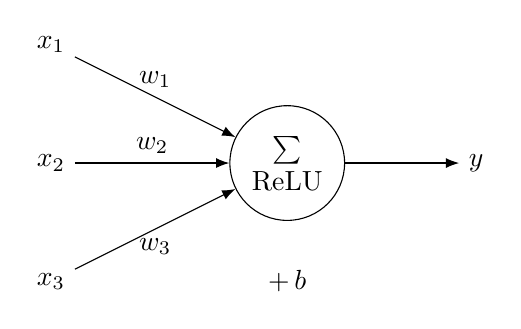
\begin{tikzpicture}[>=Latex, neuron/.style={circle, draw, minimum size=12mm}]
    \node (x1) at (0,1.5) {$x_1$};
    \node (x2) at (0,0) {$x_2$};
    \node (x3) at (0,-1.5) {$x_3$};
    \node[neuron, align=center] (n) at (3,0) {$\sum$\\ReLU};
    \node (y) at (5.4,0) {$y$};

    \draw[->] (x1) -- node[above] {$w_1$} (n);
    \draw[->] (x2) -- node[above] {$w_2$} (n);
    \draw[->] (x3) -- node[below] {$w_3$} (n);
    \draw[->] (n) -- (y);
    \node at (3,-1.5) {$+\,b$};
\end{tikzpicture}
\caption{A single neuron computes a weighted sum, adds a bias, and applies ReLU.}
\end{figure}

Let $w_1=4$, $w_2=1$, $w_3=-2$, and $b=-4$. For
$x_1=3$, $x_2=2$, and $x_3=1$,
\[
    y = \sigma(4 \cdot 3 + 1 \cdot 2 + (-2) \cdot 1 - 4)
      = \sigma(8) = 8.
\]
For $x_1=1$, $x_2=6$, and $x_3=5$,
\[
    y = \sigma(4 \cdot 1 + 1 \cdot 6 + (-2) \cdot 5 - 4)
      = \sigma(-4) = 0.
\]
The two examples use the same neuron parameters. Only the input changes, so the
weighted sum changes from a positive value to a negative value; ReLU passes the
positive value through and clips the negative value to zero.

\section{Dot Products}

The weighted sum in linear regression and in a neuron can be written as a dot
product. For two vectors
\[
    w = (w_1,\ldots,w_n), \qquad x = (x_1,\ldots,x_n),
\]
their dot product is
\[
    w \cdot x = w_1x_1 + \cdots + w_nx_n.
\]
Thus the pre-activation value of a neuron can be written compactly as
\[
    z = w \cdot x + b.
\]
The dot product measures a weighted combination of the input features.

For example, if $a = (\avec{1,2,3})$ and $b = (\bvec{4,5,6})$, then
\[
    \avec{a} \cdot \bvec{b}
    = \avec{1} \cdot \bvec{4}
    + \avec{2} \cdot \bvec{5}
    + \avec{3} \cdot \bvec{6}
    = 4 + 10 + 18 = 32.
\]

\section{Matrix-Vector Multiplication}

A layer of several neurons can be represented by a weight matrix. Suppose a
layer has $m$ neurons and each neuron receives the same input vector $x$ with
$n$ features. The weights can be arranged as a matrix
\[
    W =
    \begin{bmatrix}
    w_{11} & w_{12} & \cdots & w_{1n} \\
    w_{21} & w_{22} & \cdots & w_{2n} \\
    \vdots & \vdots & \ddots & \vdots \\
    w_{m1} & w_{m2} & \cdots & w_{mn}
    \end{bmatrix}.
\]
The product $Wx$ is a vector with one entry for each neuron:
\[
    Wx =
    \begin{bmatrix}
    w_1 \cdot x \\
    w_2 \cdot x \\
    \vdots \\
    w_m \cdot x
    \end{bmatrix}.
\]
Matrix-vector multiplication is therefore repeated dot product: The matrix is split into rows and then we calculate the dot product of the input vector and each row of the matrix.

For example, let
\[
    A =
    \begin{bmatrix}
    \rowone{1} & \rowone{2} & \rowone{3} \\
    \rowtwo{4} & \rowtwo{5} & \rowtwo{6}
    \end{bmatrix},
    \qquad
    \xvec{x} =
    \begin{bmatrix}
    \xvec{1} \\ \xvec{2} \\ \xvec{-1}
    \end{bmatrix}.
\]
Then
\[
    A\xvec{x} =
    \begin{bmatrix}
    \rowone{1} \cdot \xvec{1}
    + \rowone{2} \cdot \xvec{2}
    + \rowone{3} \cdot \xvec{(-1)} \\
    \rowtwo{4} \cdot \xvec{1}
    + \rowtwo{5} \cdot \xvec{2}
    + \rowtwo{6} \cdot \xvec{(-1)}
    \end{bmatrix}
    =
    \begin{bmatrix}
    \rowone{2} \\ \rowtwo{8}
    \end{bmatrix}.
\]

\section{Layer Calculations as Matrix Operations}

Using matrices, the computation of an entire layer can be written as
\[
    z = Wx + b,
\]
where $b$ is now a vector of bias terms. The activation function is then applied
component by component:
\[
    a = f(z).
\]
For ReLU, this means applying $\max(0,z_i)$ to each component $z_i$.

A neural network consists of several such layers. If $a^{(0)} = x$ is the input,
then a typical layer computes
\[
    z^{(\ell)} = W^{(\ell)}a^{(\ell-1)} + b^{(\ell)}, \qquad
    a^{(\ell)} = f(z^{(\ell)}).
\]
This notation shows why matrix-vector multiplication is central to neural
networks: it computes all weighted sums in a layer at once. Modern hardware can
perform these matrix operations efficiently, which is one reason neural networks
scale to large models and large datasets.

\section{Example: A Two-Layer Network}

Consider a network with input
\[
    x =
    \begin{bmatrix}
    2 \\ 3
    \end{bmatrix},
    \qquad
    W_1 =
    \begin{bmatrix}
    1 & 4 \\
    0 & -3
    \end{bmatrix},
    \qquad
    W_2 =
    \begin{bmatrix}
    -2 & 7 \\
    3 & -9
    \end{bmatrix}.
\]
Use bias vectors
\[
    b^{(1)} =
    \begin{bmatrix}
    -2 \\ 1
    \end{bmatrix},
    \qquad
    b^{(2)} =
    \begin{bmatrix}
    3 \\ 4
    \end{bmatrix},
\]
and apply ReLU after each layer.
\begin{figure}[h]
\centering
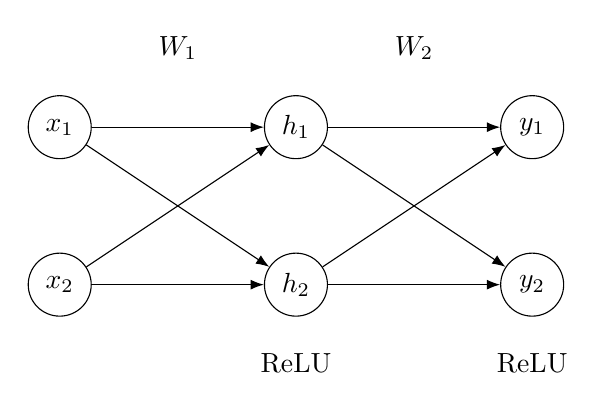
\begin{tikzpicture}[>=Latex, neuron/.style={circle, draw, minimum size=8mm}]
    \node[neuron] (x1) at (0,1) {$x_1$};
    \node[neuron] (x2) at (0,-1) {$x_2$};

    \node[neuron] (h1) at (3,1) {$h_1$};
    \node[neuron] (h2) at (3,-1) {$h_2$};

    \node[neuron] (y1) at (6,1) {$y_1$};
    \node[neuron] (y2) at (6,-1) {$y_2$};

    \foreach \i in {x1,x2}
        \foreach \j in {h1,h2}
            \draw[->] (\i) -- (\j);

    \foreach \i in {h1,h2}
        \foreach \j in {y1,y2}
            \draw[->] (\i) -- (\j);

    \node at (1.5,2) {$W_1$};
    \node at (4.5,2) {$W_2$};
    \node[align=center] at (3,-2) {ReLU};
    \node[align=center] at (6,-2) {ReLU};
\end{tikzpicture}
\caption{A two-layer fully connected neural network with two input units, two
hidden units, and two output units.}
\end{figure}

The first layer computes
\[
    z^{(1)} = W_1x + b^{(1)} =
    \begin{bmatrix}
    1 & 4 \\
    0 & -3
    \end{bmatrix}
    \begin{bmatrix}
    2 \\ 3
    \end{bmatrix}
    +
    \begin{bmatrix}
    -2 \\ 1
    \end{bmatrix}
    =
    \begin{bmatrix}
    1 \cdot 2 + 4 \cdot 3 - 2 \\
    0 \cdot 2 + (-3) \cdot 3 + 1
    \end{bmatrix}
    =
    \begin{bmatrix}
    12 \\ -8
    \end{bmatrix}.
\]
After ReLU,
\[
    a^{(1)} = \operatorname{ReLU}(z^{(1)}) =
    \begin{bmatrix}
    12 \\ 0
    \end{bmatrix}.
\]

The second layer computes
\begin{align*}
    z^{(2)}
    &= W_2a^{(1)} + b^{(2)} \\
    &=
    \begin{bmatrix}
    -2 & 7 \\
    3 & -9
    \end{bmatrix}
    \begin{bmatrix}
    12 \\ 0
    \end{bmatrix}
    +
    \begin{bmatrix}
    3 \\ 4
    \end{bmatrix}
    \\
    &=
    \begin{bmatrix}
    (-2) \cdot 12 + 7 \cdot 0 + 3 \\
    3 \cdot 12 + (-9) \cdot 0 + 4
    \end{bmatrix}
    \\
    &=
    \begin{bmatrix}
    -21 \\ 40
    \end{bmatrix}.
\end{align*}
Applying ReLU again gives the network output
\[
    y = \operatorname{ReLU}(z^{(2)}) =
    \begin{bmatrix}
    0 \\ 40
    \end{bmatrix}.
\]

\section{Tensors}

In machine learning, a \emph{tensor} is a structured container for numerical
data. It is used in many machine learning frameworks such as PyTorch and Tensorflow.
  Scalars, vectors, matrices, and higher-dimensional arrays can all be
viewed as tensors. The number of dimensions is often called the tensor's
\emph{rank} or \emph{order}. In PyTorch, tensors are represented with
\texttt{torch.Tensor} objects.

\begin{figure}[h]
\centering
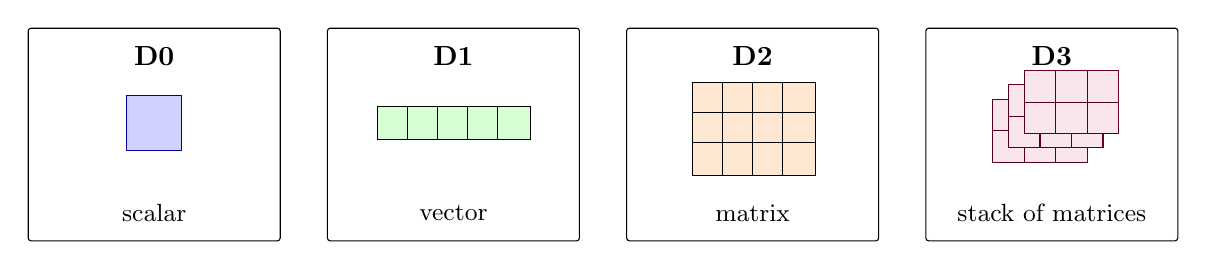
\begin{tikzpicture}[
    tensorbox/.style={draw, rounded corners=1pt, minimum width=3.2cm,
        minimum height=2.7cm},
    cell/.style={draw, minimum width=0.42cm, minimum height=0.42cm},
    every node/.style={font=\small}
]
    \node[tensorbox] (d0box) at (0,0) {};
    \node[font=\bfseries] at (0,1.0) {D0};
    \node at (0,-1.0) {scalar};
    \draw[fill=blue!18, draw=blue!60!black] (-0.35,-0.2) rectangle (0.35,0.5);
    % \draw[fill=blue!10, draw=blue!60!black] (-0.35,0.5) -- (-0.12,0.73) -- (0.58,0.73) -- (0.35,0.5) -- cycle;
    % \draw[fill=blue!25, draw=blue!60!black] (0.35,-0.2) -- (0.58,0.03) -- (0.58,0.73) -- (0.35,0.5) -- cycle;

    \node[tensorbox] (d1box) at (3.8,0) {};
    \node[font=\bfseries] at (3.8,1.0) {D1};
    \node at (3.8,-1.0) {vector};
    \foreach \i in {0,...,4} {
        \node[cell, fill=green!16] at (3.05+0.38*\i,0.15) {};
    }

    \node[tensorbox] (d2box) at (7.6,0) {};
    \node[font=\bfseries] at (7.6,1.0) {D2};
    \node at (7.6,-1.0) {matrix};
    \foreach \r in {0,...,2} {
        \foreach \c in {0,...,3} {
            \node[cell, fill=orange!18] at (7.05+0.38*\c,0.45-0.38*\r) {};
        }
    }

    \node[tensorbox] (d3box) at (11.4,0) {};
    \node[font=\bfseries] at (11.4,1.0) {D3};
    \node at (11.4,-1.0) {stack of matrices};
    \foreach \s/\dx/\dy in {0/0.00/0.00,1/0.20/0.18,2/0.40/0.36} {
        \draw[fill=purple!10, draw=purple!55!black] (10.65+\dx,-0.35+\dy) rectangle (11.85+\dx,0.45+\dy);
        \foreach \r in {0,1} {
            \draw[purple!45!black] (10.65+\dx,-0.35+\dy+0.4*\r) -- (11.85+\dx,-0.35+\dy+0.4*\r);
        }
        \foreach \c in {0,1,2} {
            \draw[purple!45!black] (10.65+\dx+0.4*\c,-0.35+\dy) -- (10.65+\dx+0.4*\c,0.45+\dy);
        }
    }
\end{tikzpicture}
\caption{Different types of $N$-dimensional tensors from $N=0$ to 3. There is
no limit to the value of $N$.}
\end{figure}

A 0D tensor is a scalar tensor. In the PyTorch example below,
\texttt{torch.tensor(3.14)} creates a tensor that contains the single value
\texttt{3.14} and has no axes. Therefore its shape is \texttt{torch.Size([])},
not \texttt{[1]}.
\begin{verbatim}
import torch

x0 = torch.tensor(3.14)
print(x0.shape)  # torch.Size([])
\end{verbatim}

A 1D tensor is a vector, such as a list of input features.
\begin{verbatim}
x1 = torch.tensor([5.0, 12.0, 15.0])
print(x1.shape)  # torch.Size([3])
\end{verbatim}

A 2D tensor is a matrix. For example, a weight matrix can map several input
features to several neurons.
\begin{verbatim}
x2 = torch.tensor([
    [1.0, 2.0, 3.0],
    [4.0, 5.0, 6.0],
])
print(x2.shape)  # torch.Size([2, 3])
\end{verbatim}

A 3D tensor can represent a batch of matrices. A \emph{batch} is a group of
examples processed together in one computation. For example, three grayscale
images of size $4 \times 4$ can be stored with shape \texttt{[3, 4, 4]}. In this
case, the batch size is 3, and each example in the batch is a $4 \times 4$
matrix.
\begin{verbatim}
x3 = torch.zeros(3, 4, 4)
print(x3.shape)  # torch.Size([3, 4, 4])
\end{verbatim}

A 4D tensor is common in image processing, where data is often organized as
\texttt{[batch, channels, height, width]}. For example, a batch of eight RGB
images of size $32 \times 32$ has shape \texttt{[8, 3, 32, 32]}.
\begin{verbatim}
x4 = torch.zeros(8, 3, 32, 32)
print(x4.shape)  # torch.Size([8, 3, 32, 32])
\end{verbatim}

Tensors are central in neural networks because inputs, outputs, weights,
activations, gradients, and batches of training examples are all represented as
tensors. Neural network libraries such as PyTorch are designed to perform tensor
operations efficiently and to compute gradients through those operations.

Modern GPUs process tensors by storing them as arrays in memory and applying
many small arithmetic operations in parallel. In practice, high-level tensor
operations are usually decomposed into matrix multiplication, convolution, and
elementwise kernels. Since NVIDIA's Volta architecture in 2017, many GPUs have
also included dedicated \emph{Tensor Cores}, hardware units designed to
accelerate small matrix multiply-accumulate operations used in neural
networks.\footnote{\url{https://developer.nvidia.com/blog/programming-tensor-cores-cuda-9/}}
Thus, although programmers work with tensors of different ranks, the hardware
often executes tiled matrix operations and related parallel kernels.

\section{Summary}

Linear regression predicts a numeric value using a weighted sum of input
features. A neuron generalizes this idea by applying an activation function to
the weighted sum. ReLU is a simple nonlinear activation that returns zero for
negative inputs and the input itself for positive inputs. Dot products express
weighted sums compactly, and matrix-vector multiplication computes many dot
products at once. Neural network layers are therefore naturally represented as
matrix-vector calculations followed by nonlinear activation functions.


\chapter{Gradient Descent}


\end{document}
